\documentclass[prl,showpacs]{revtex4-1}
\usepackage{graphicx,amssymb,color}
\usepackage[dvipsnames]{xcolor}
%\usepackage[utf8]{inputenc}
\usepackage[spanish]{babel}


\begin{document}
\title{FI3104 M\'etodos N\'umericos para la Ciencia e Ingenieria\\ Tarea 6}
\author{Camila Sandivari}
\affiliation{Profesor: Valentino Gonzalez \\ Profesor Auxiliar: Felipe Pesce}
\date{\today}

\begin{abstract}
El presente reporte muestra la resoluci\'on de ecuaciones parab\'olicas, que modelan procesos de reacci\'on y difusi\'on para dos sistemas de inter\'es; Fisher-KPP modela como una onda la forma en que un gen se dispersa espacialmente en una poblaci\'on, cuando \'este es ventajoso para la especie, Newell-Whitehead-Segel describe convecci\'on de la forma Rayleigh-Benard que se produce en una capa de fluido calentada desde abajo.
Para lograr el objetivo se debe discretizar usando m\'etodos distintos, la parte de la reacci\'on se resuelve con un m\'etodo de Euler expl\'icito y la parte de la difusi\'on con Cranck-Nickolson. 

\end{abstract}
\maketitle


\paragraph{Procedimiento}
\subparagraph{Parte 1}
Para resolver la ecuaci\'on de Fisher-KPP (1) con sus respectivas condiciones iniciales, se implementa un algoritmo que resuelve la parte de difusi\'on con m\'etodo Cranck-Nickolson y la de reacci\'on con m\'etodo Euler expl\'icito. 

\begin{equation}
\frac{\partial n}{\partial t} = \gamma \frac{\partial^2n}{\partial x^2} + \mu n - \mu n^2
\end{equation}
\begin{eqnarray}
 n(t, 0) &= 1\\ n(t, 1) &= 0\\ n(0, x) &= e^{-x^2/0.1} 
\end{eqnarray}

Con $n(x,t)$ la densidad de la especie en tiempo , $\mu n$ la tendencia de la especie a crecer indefinidamente, $-\mu n^{2}$ el factor competencia debido al aumento de densidad de poblaci\'on, y $\gamma \nabla n$ la tendencia de la especie a dispersarse para encontrar m\'as recursos.\\
Los m\'etodos de resoluci\'on se obtienen de resolver la ecuaci\'on (5) mediante discretizar de la forma mostrada en (6). Cuando el par\'ametro a es igual a 0 se tiene el m\'etodo de Euler expl\'icito que resuelve la parte de reacci\'on del problema, y cuando a igual a 1 se conoce como m\'etodo Cranck-Nickolson y resuelve la parte de difusi\'on del problema.
\begin{center}
\begin{equation}
\frac{\partial T}{\partial t} = \frac{\partial^2 T}{\partial x^2}
\end{equation}
\end{center}
\begin{equation}
\frac{T^{n+1}_{k} - T^{n}_{k}}{\epsilon} =\\
 \frac{a}{2} \left[ \frac{T^{n+1}_{k+1} - 2T^{n+1}_{k}+T^{n+1}_{k-1}}{h^{2}}\right] +  \frac{2-a}{2} \left[ \frac{T^{n}_{k+1} - 2T^{n}_{k}+T^{n}_{k-1}}{h^{2}}\right]
\end{equation}

El algoritmo implementado busca resolver ecuaciones parab\'olicas lineales, asumiendo que son de la forma $A\overrightarrow{\varphi}=\overrightarrow{b}$ y buscando los par\'ametros que la ajustan a los casos particulares de cada problema a resolver.

\subparagraph{Parte 2}
El problema dos es an\'alogo al anterior pero se busca resolver el siguiente sistema, correspondiente a la ecuaci\'on Newell-Whitehead-Segel:

\begin{equation}
\frac{\partial n}{\partial t} = \gamma \frac{\partial^2n}{\partial x^2} + \mu ( n - n^3)
\end{equation}
\begin{eqnarray}
n(t, 0) &= 0\\ n(t, 1) &= 0\\ n(0, x) &= \texttt{np.random.uniform(low=-0.3, high=0.3, size=Nx)}
\end{eqnarray}

\paragraph{Resultados}
\subparagraph{Parte 1}

Se presenta en la figura 1 el gr\'afico para la densidad $n(x,t)$ en funci\'on de x, la posici\'on. Se observa el equilibrio inestable en $x = 0$ porque corresponde a un m\'aximo en la funci\'on y un equilibrio estable en $x =1$ que se v\'e como el m\'inimo.

\begin{figure}
\begin{center}
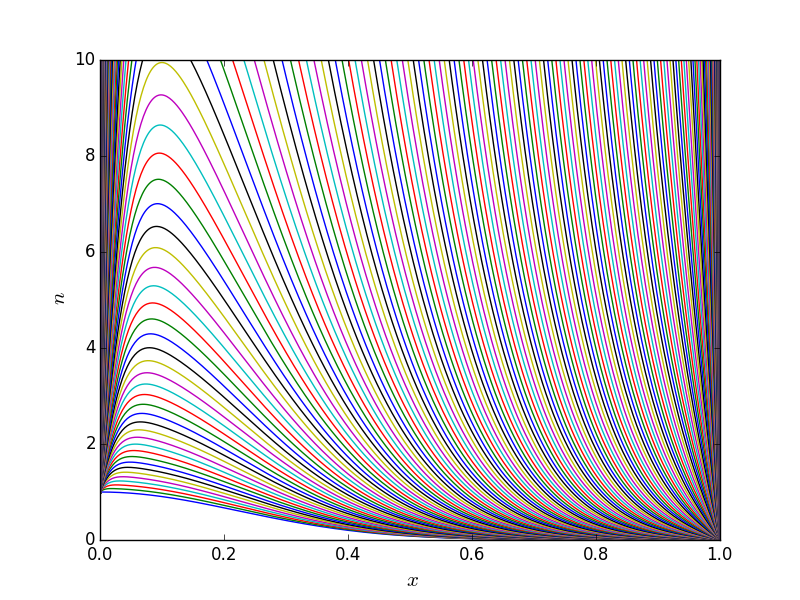
\includegraphics[width=5in]{p1.png}
\caption{ Densidad de poblaci\'on obtenida de la ecuaci\'on Fisher- KPP.En el eje y se encuentra la densidad. En el eje x se encuentra la variable x referente a la posici\'on. }
\label{ }
\end{center}
\end{figure}

\subparagraph{Parte 2 }
Los gr\'aficos de las figuras 3 y 4 presentan la soluci\'on de la densidad para la ecuaci\'on Newell-Whitehead-Segel, y la representaci\'on en mapa de colores de x versus t, respectivamente. Se observan los puntos de equilibrio previstos, $x=0$ y $x=\pm 1$. 
\begin{figure}
\begin{center}
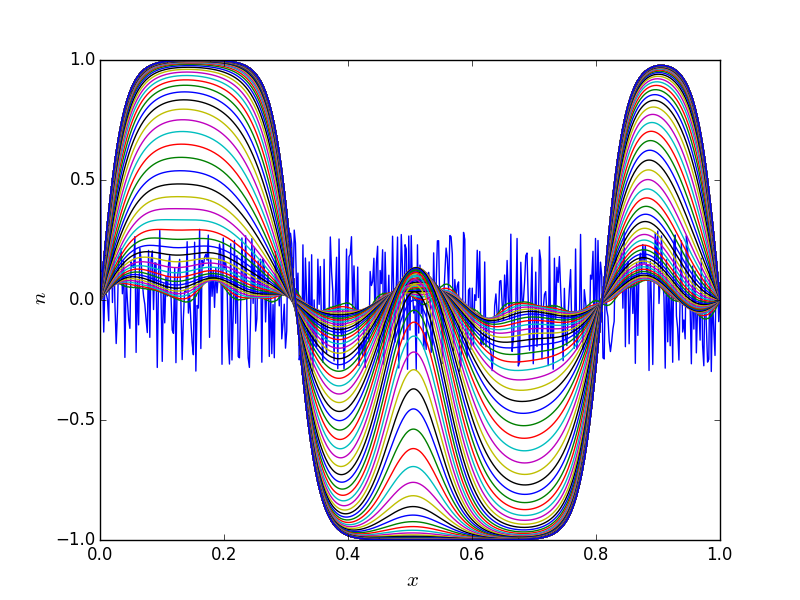
\includegraphics[width=5in]{p2.png}
\caption{ Densidad de poblaci\'on obtenida de la ecuaci\'on Newell-Whitehead-Segel .En el eje y se encuentra la densidad. En el eje x se encuentra la variable x referente a la posici\'on.}
\label{ }
\end{center}
\end{figure}

\begin{figure}
\begin{center}
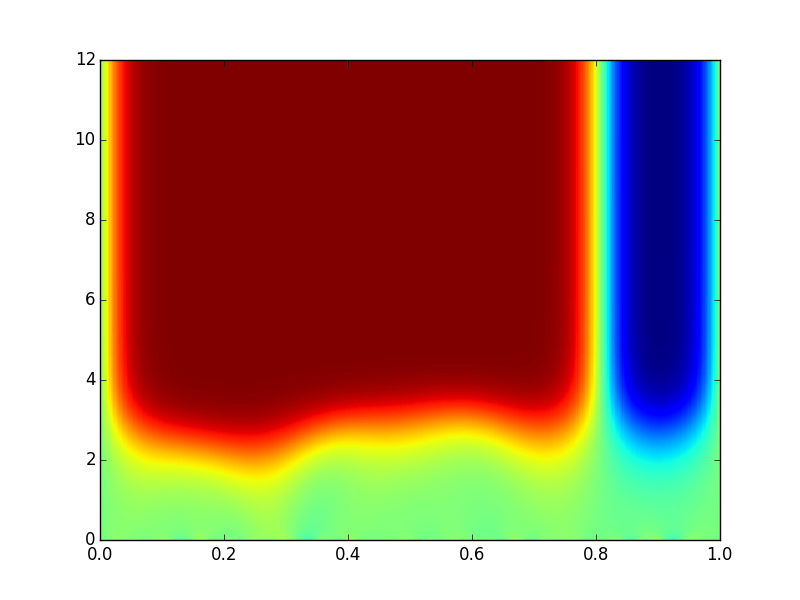
\includegraphics[width=5in]{p2lindo.png}
\caption{ Mapa a color de x versus t. En el eje y se ve la posici\'on x. En el eje x se ve el tiempo }
\label{ }
\end{center}
\end{figure}

\newpage
\paragraph{Conclusiones}
Se logran resolver las ecuaciones planteadas, usando el m\'etodo tridiagonal para ecuaciones parab\'olicas,dividido en Euler expl\'icito y Cranck- Nickolson dependiendo de la etapa estudiada, entendiendo que se estudian ecuaciones que describen procesos de difusi\'on y reacci\'on. Se obtiene una idea clara de la evoluci\'on de los sistemas, sus puntos de equilibrio y respectivas estabilidades a trav\'es de graficos de la densidad en funci\'on de la posici\'on.


\end{document}